\documentclass{article}

\title{Semestrální projekt LAR}
\author{Matěj Pinkas, Martin Erben, Filip Hudec}
\date{27.3.2024}

\usepackage[a4paper, includehead,left=2.1cm,
    		right=2.1cm,top=2.4cm,
    		bottom=2.4cm]{geometry}
\usepackage{fancyhdr}
\usepackage{pagecolor}
\usepackage{sectsty}
\usepackage{amsmath}
\usepackage{amssymb}
\usepackage{bbold}
\usepackage[colorlinks=true,linkcolor=red]{hyperref} % for hyperlinks
\usepackage{graphicx}
\usepackage{caption}
\usepackage{varioref} % Load the varioref package
\usepackage{subcaption}
\usepackage{bm} % Bold text in mathmode
\usepackage{enumitem}
\usepackage{gensymb}

\renewcommand{\contentsname}{Obsah}
\captionsetup[table]{name=Tab.}
\captionsetup[figure]{name=Obr.}

\begin{document}

\pagecolor{white}
\pagestyle{fancy}

\fancyhead{} % clear all header fields
\fancyhead[L]{M. Pinkas, M. Erben, F. Hudec}
\fancyhead[C]{Semestrální projekt LAR}
\fancyhead[R]{B3B33LAR}

\maketitle

\tableofcontents
\clearpage

\section{Úvod}
Tento projekt slouží jako výstup z předmětu LAR. Cílem je projet stanovenou dráhu s robotem v časovém limitu, kde se bude pohybovat zcela autonomně podle barevných směrovek. Pro splnění tohoto úkolu používáme platformu TurtleBot. Jedná se ve stručnosti o hnaný dvoukolový podvozek, který je doplněn o nástavbu s osazenými senzory (více v sekci \ref{sssec:1}). Směrovky jsou tvořeny dvojicí barevných sloupků.\\
Na výběr jsme dostali ze tří zadání podle úrovně obtížnosti. Náš tým si vybral 2. možnost - průjezd tratě bez překážek s tím, že přidáme zastavení u poslední dvojice zelených sloupků.

\section{Rozbor problému}
Robot je nejdříve umístěn na startovní pozici, ve výseči první směrovky $\pm 45$\degree{}, která má vrchol ve středu směrovky. Vzdálenost start – první ukazatel leží v intervalu $(a; b) = (500; 3000)$ mm. Robot může být libovolně natočen, takže si musí první směrovku najít s tím, že volí tu nejblíže k němu.\\
Poté, co spustíme na robotovi program a cvičící stiskne tlačítko pro zahájení pohybu, již nemůžeme robota externě ovládat a musí se rozhodovat autonomně.\\
Pro případ, že by došlo k chybě (tj. nárazu do jakékoliv překážky) je robot vybaven nárazníkem, který pošle callback řídícímu programu a ten je okamžitě ukončen.\\
Naše použité směrovky jsou tvořeny modrým a červeným sloupkem. Jejich rozestup je specifikován\\na $50\pm5$ mm.\\
Při navigaci od aktuální k následující směrovce musí spojnice středů těchto směrovek s osou následující směrovky vždy svírat úhel $\delta \leq 45$\degree{}. Následující směrovka leží vždy vpravo nebo vlevo od aktuální a to ve výseči $\rho=90$\degree{}, která začíná od úhlu $\beta=45$\degree{} měřeno od osy aktuální směrovky (viz Obr. \ref{fig:1}).\\
Časový limit na kompletní průjezd je v této úloze stanoven na 5 min.
	\begin{figure}[h!]
        		\centering
        		\setlength{\unitlength}{1cm}
    		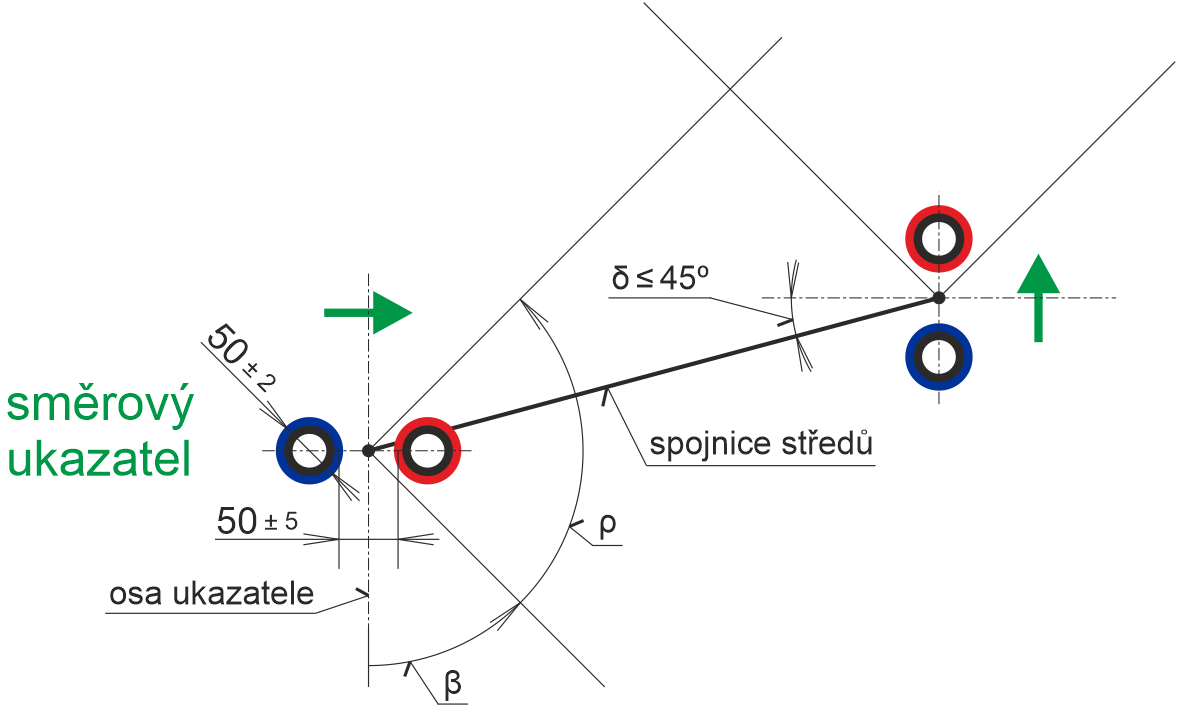
\includegraphics[width=0.6\textwidth]{vykres_ukazatel_jizda.png}
        		\caption{Parametry vyznačené tratě}
		\label{fig:1}
    	\end{figure}

	\subsection{Návrh řešení}
	Při spuštění programu si robot inicializuje RGB a 3D hloubkovou kameru. Na obrazovce počítače, ze kterého spouštíme řídicí program zobrazujeme 4 okna (viz Obr. \ref{fig:2}): obraz z hloubkové kamery; obraz z RGB kamery; obraz z RGB kamery s vymaskovanými směrovkami a našemi navigačními body; mapa zobrazující výseč prostoru, kterou robot snímá (top-down view). \\
	Robot si uloží 2 nebližší směrovky, které vidí, podle dat z RGB a hloubkové kamery. Vybere z nich tu bližší a spočítá si 3 virtuální body (M, T, P), podle kterých se bude navigovat k nejbližší směrovce. \\
	Bod M leží v polovině spojnice středů dvou sloupků. Bod T (\textit{target}) leží na kolmici ke spojnici středů sloupků (kde bod M je průsečík těchto přímek) ve vzdálenosti $50\pm5$ mm od sloupků a je to bod na který se snažíme dostat tak, aby ještě robot neshodil sloupky. Bod P potom leží na stejné kolmici jako T a M, ale leží ve vzdálenosti 100 mm od sloupků. \\
	Robot si uloží z odometrie počáteční bod (resetuje odometrii) a orientuje se nejdříve na bod P, ke kterému se kolmo natočí ze své pozice a potom se k němu pohybuje již po přímce. Zde se natočí kolmo ke sloupkům a pomocí drobných translačních a rotačních pohybů se snaží dostat na požadovaný bod T. Robot se otočí podle směrovek o 90\degree a celý proces iteruje dokud se nedostane k zelené směrovce.
	\begin{figure}[h!]
        		\centering
        		\setlength{\unitlength}{1cm}
    		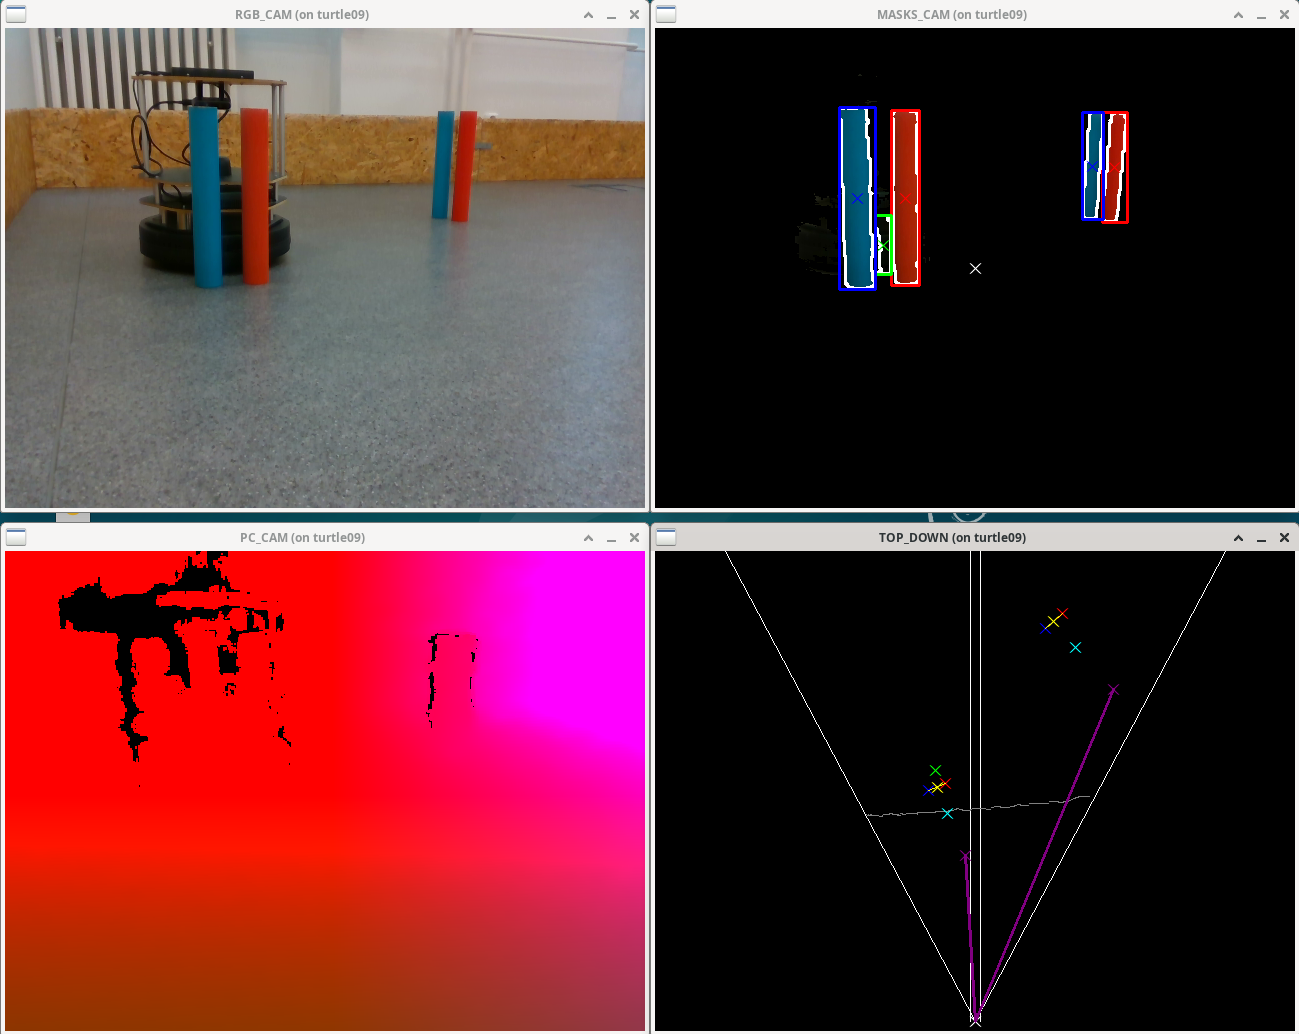
\includegraphics[width=0.6\textwidth]{all.png}
        		\caption{Obraz z pohledu robota}
		\label{fig:2}
    	\end{figure}
	
	\subsection{Očekávaná funkčnost}
	Robot by neměl mít problém se změnou osvětlení prostředí, protože při výpočtu masek pro RGB obraz naše funkce \textit{drawMasks} upravuje výchozí přednastavený rozsah barev dynamicky podle dat získaných z RGB kamery. Největším problémem kterému jsme čelili, je relativně velká nepřesnost odometrických dat, získaných z motorů robota, což nás při řízení pohybu nutilo k použití experimentálně zjišťovaných konstant, které přesně neodpovídali našim teoretickým očekávaným výsledkům. Podobně bylo třeba upravovat i data získaná z hloubkové kamery, aby jsme docílili požadovaného chování.
	
\section{Řešení problému}
	
	\subsection{Matematický model}
	
	\subsection{Algoritmizace}
	
\section{Implementace}

	\subsection{Hardware \& programovací jazyk} \label{ssec:6}
		
		\subsubsection{Platforma TurtleBot} \label{sssec:1}
		Jak už jsme zmínili, používáme open-source platformu TurtleBot 2.0 s podvozkem od firmy Kobuki. Podvozek je vybaven dvěma hnanými koly, z nichž odečítá odometrická data (natočení kol). Dále má na čelní straně blatník, který se dá zmáčknout ve třech segmentech (Right, Left, Center) a v případě srážky s překážkou pošle callback, kterým můžeme zastavit chod řídicího programu. \\
		V nástavbě se schovává počítač Intel NUC, na kterém běží operační systém Linux, a v němž spouštíme náš řídicí program prostřednictvím virtualizace Singularity. Dále zde najdeme senzor Intel RealSense D435/D435i, který obsahuje RGB kameru s rozlišením 640x480 px a 3D hloubkovou kameru se stejným rozlišením.
		
		\subsubsection{Python}
		Celý řídicí program je implementovaný v programovacím jazyce Python. Jedná se o interpretovaný jazyk, což požaduje instalaci interpreteru v místě, kde chceme spouštět program. S robotem komunikujeme voláním jeho třídy \textit{TurtleBot}, která je implementována v dodaném balíčku \textit{robolab\_turtlebot}. Pro zpracování obrazu používáme knihovnu \textit{cv2} a pro matematické operace knihovnu \textit{NumPy}.
		
		
	\subsection{Detaily implementace}
	
	
	

\section{Závěr}

\section{Literatura}

\end{document}